%% examples.tex

%% Example 3.1
In computer graphics, 3D objects can often be parametrized by functions.
Moreover, low to medium accuracy interpolation is usually sufficient to project
satisfactory visual preceptions. In the following example, we use \funappxg to
interpolate the surface of a seashell, leading to a sufficiently accurate
three-dimensional reconstruction.

\begin{figure}[tbh]
  \centering
  \begin{tabular}{cc}
     \includegraphics[width=30mm]{figure/funappxseashell.pdf} 
  & \includegraphics[width=70mm]{figure/seashellsurferror.pdf}
  \\ a)  & b) 
  \end{tabular}
\caption{a) Approximate seashell; b) Error estimation of seashell with tolerance
$0.1$. This figure is reproducible by \texttt{traub\_funappxseashell.m}.}
\label{fig:funappxseashell}
\end{figure}
\begin{exmp}
 
Figure~\ref{fig:funappxseashell}a) is an approximation of a 
seashell portrayed as a parametric surface in 3D. Let $a=-0.2$, $b=0.5$,
$c=0.1$, $n = 2$, $u,v \in [0, 2 \pi]$, and $w(v) =
a\left(1-\frac{v}{2\pi}\right)$. The parametric surface is defined by the
following equations in~\cite{DavEtal05}:
\begin{align*}
x(u,v) & =   \left[ w(v) \left(1+\cos(u)\right) + c\right]\cos(nv),\\
y(u,v) & = \left[w(v) (1+\cos(u)) + c\right] \sin(nv),\\
z(u,v) & = {bv}/{2\pi} + w(v)\sin(u).
\end{align*}
%
\begin{comment}
If a function of two variables $f(x,y)$ can be separated, such as
$$f(x,y)=f_1(x)+f_2(y) \text{ or } f(x,y)=f_1(x)f_2(y),$$ we can apply
\texttt{funappx\_g} directly to $f_1(x)$ and $f_2(y)$. However, $x(u,v)$,
$y(u,v)$, and $z(u,v)$ can not be represented by the form mentioned above.
Instead,
\end{comment}
%We approximate $\sin(x)$ and $\cos(x)$ on the interval $[0,4\pi]$. Denote
Denote $\sinappx(x)$ and $\cosappx (x)$ the approximate functions of $\sin(x)$ and
$\cos(x)$ on the interval $[0,4\pi]$, respectively; and let the resultant
approximants of $x(u,v)$, $y(u,v)$, and $z(u,v)$ be $\hat{x}(u,v)$,
$\hat{y}(u,v)$, and $\hat{z}(u,v)$, respectively.
\begin{comment}
Then we have
\begin{align*}
   \hat{x}(u,v) & =  \left[a\left(1-\frac{v}{2\pi}\right)\left(1+\cosappx(u)\right) + c\right]\cosappx(nv),
\\ \hat{y}(u,v) & = \left[a\left(1-\frac{v}{2\pi}\right)(1+\cosappx(u)) + c\right] \sinappx(nv),
\\ \hat{z}(u,v) & = \frac{bv}{2\pi} + a\left(1-\frac{v}{2\pi}\right)\sinappx(u).
\end{align*}
\end{comment}
Define the overall approximation error measure as
\begin{align*}
\mathscr{E} =  \max\limits_{u,v \in [0, 2 \pi] } & \left\{   |x(u,v)-\hat{x}(u,v)|,\right.
   \left.  |y(u,v)-\hat{y}(u,v)|, 
                                  \ \    |z(u,v)-\hat{z}(u,v)|\right\}.
\end{align*}
Even if we set the error tolerance $\abstol$ to be as big as $0.1$ for computing
$\sinappx$ and $\cosappx$, we can still obtain a much diminished error
$\mathscr{E}\approx 9 \times 10^{-4}$; see the error plot in
Figure~\ref{fig:funappxseashell}b). The reconstructed surface in
Figure~\ref{fig:funappxseashell}a) is very similar to the original seashell
image.
\end{exmp}

In digital animation, frames of images are produced to represent movements of
objects over small discrete time. To automatically insert additional frames between 
two consecutives frames for better visual effects, temporal
interpolation can often be applied to estimate an object's positions by using
parametric curves that represent its trajectory in 3D as $(x(t), y(t), z(t))$,
where each Cartesian coordinate in space is parametrized by time $t$. We refer
readers to Example~5 in \cite[Chapter~3, Section~6]{Din15a} for an illustration.

%% Example 3.2

The next example showcases the merits and demerits of our algorithm and an
existing method for high-accuracy function approximation.

\begin{exmp}
Chebfun~\cite{TrefEtal15a} is a MATLAB toolbox known for using Chebyshev
polynomial basis for approximating given functions to machine precision
($\approx 10^{-15}$). In this example, we show that it is challenged by~$f_3$
defined in Section~\ref{sec:cone}. Around $x=0$ and $x=0.2$, some pointwise
errors of the piecewise Chebyshev interpolant spike to more than $10^{-5}$ as
shown in Figure~\ref{f3chebfig}a). Regretably Chebfun did not issue any warning
about the inaccurate representation in this case. In contrast, the errors of the
piecewise linear interpolant from \funappxg{} are uniformly below $10^{-14}$.
Nonetheless the time taken by \funappxg{} was close to 7 seconds for such an 
accurate approximation.

%
\begin{figure}[tbh]
\centering
\begin{tabular}{cc}
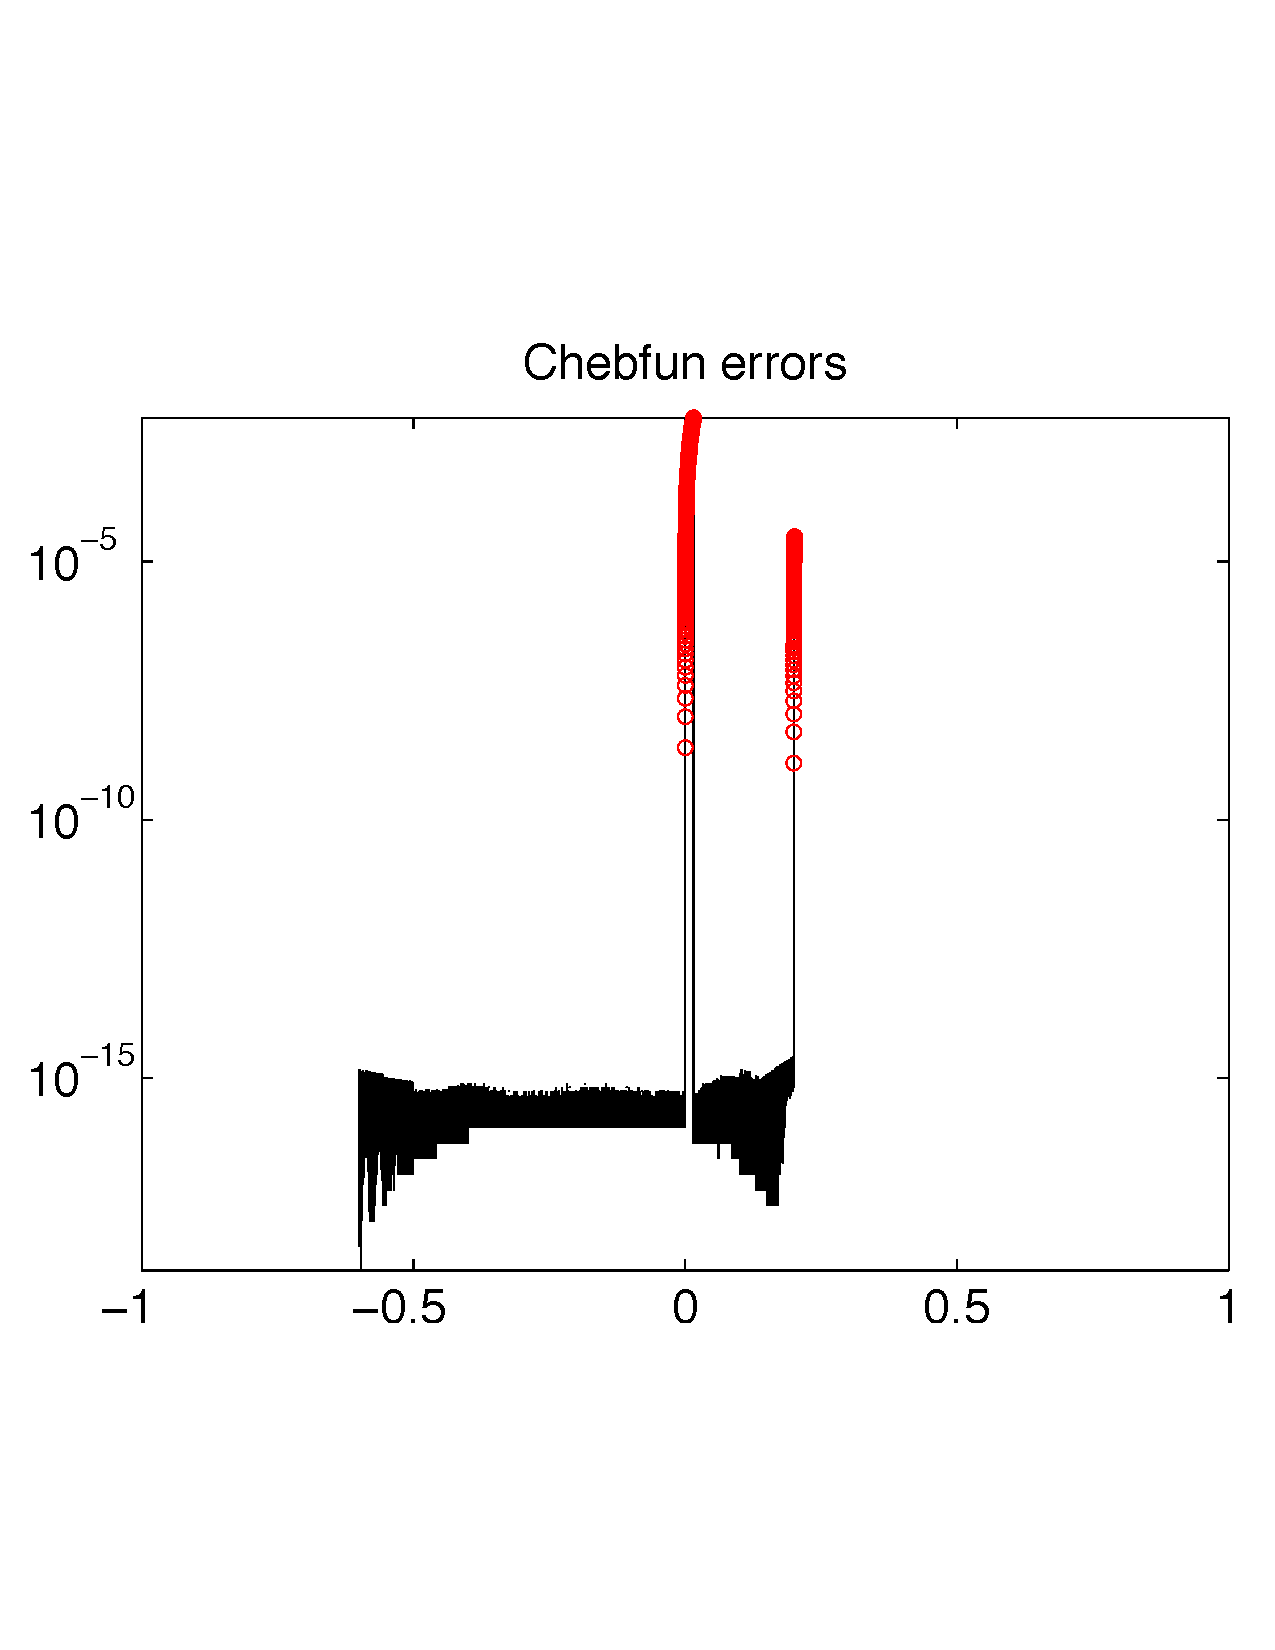
\includegraphics[width=5.9cm]{figure/chebfun_errors.pdf} \hspace{-2ex} &
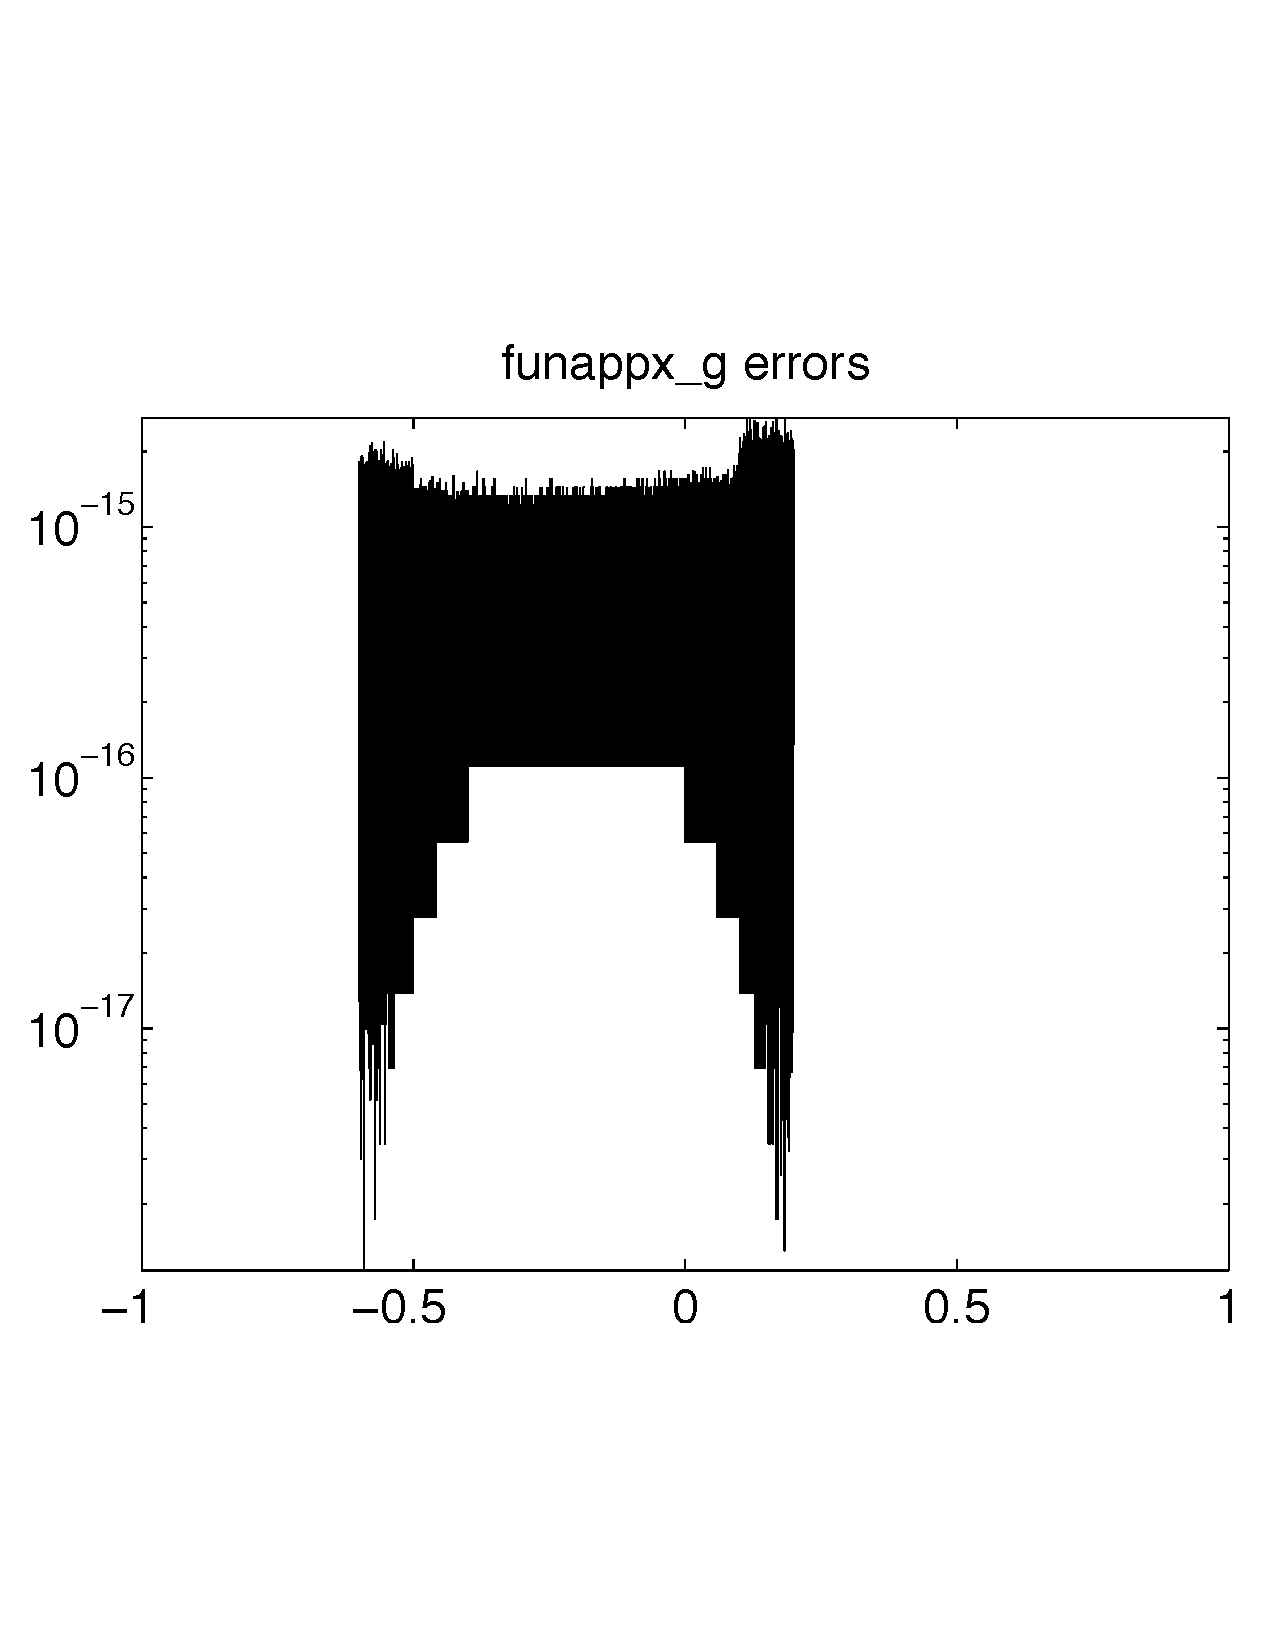
\includegraphics[width=5.9cm]{figure/funappx_g_errors.pdf}
\\ a) & b)
\end{tabular}
\caption{Approximating $f_3(x)$ with errors of interpolants returned from a)
Chebfun and b) \funappxg. This figure is reproducible by
\texttt{cf\_chebfun.m}. \label{f3chebfig}}
\end{figure}
%

\end{exmp}

\begin{comment}
Our algorithm is readily extensible to the following complex-valued function.
\begin{exmp} This example is taken from MATLAB's documentation for
\texttt{interp1}. Define the complex valued function $v(x) = 5x + x^2 i$ for $x
\in [1,10]$. It is clear that the real part of $v$ is $5x$ and the imaginary
part is $x^2$. We could apply \funappxg to approximate the two parts separately.
However, it is unnecessary.
\end{exmp}
\end{comment}

%% Example 3.3

\begin{exmp}
In this example, we want to compare our adaptive algorithms with Chebfun by
simulating the following families of test functions:

\begin{align*}
 g_1(x) &= x^4 \sin(d/x), \qquad
 g_2(x) = 10  x^2 + g_1(x),
\\ g_3(x) &= \begin{cases} \displaystyle
   \frac{1}{2\delta^2} \Bigl [4 \delta^2 + (x-c)^2 + (x-c-\delta)\abs{x-c-\delta}
\\ \qquad \qquad
    - (x-c+\delta)\abs{x-c+\delta} \Bigr ], & \abs{x-c} \le 2\delta,
\\ 0, & \text{otherwise},
\end{cases} \\
 g_4(x) & = (x-d)^2, \qquad
 g_5(x)= d\sin(d\pi x), \qquad
 g_6(x)= 10\exp\left(-1000(x-d)^2\right), \qquad
% \\ f_4(x)&= \frac{c}{4}\exp(-2x)(c-2\exp(x)(-1 + c\cos(x) - c\sin(x)) \\
%  & \ \ +\exp(2x)(c + 2\cos(x)- 2\sin(x) - c\sin(2x))),
\end{align*}
where $c$ for defining $g_3$ is uniformly drawn $100$ times from $[0,0.6]$ and
$d$ for other functions from $[0,4]$. If $c=d=1$, then $g_i$ reduces to $f_i$
for $i=1,2, \mbox{and } 3$. Figure~\ref{fig:testfunctions}a) shows the shapes of
the test functions when $c=2.5$ and $d=0.375$. We set $\abstol = 10^{-6}$ and
use \texttt{funappx\_g} and \texttt{funappxglobal\_g} to approximate the test
functions on interval $[a,b]=[0,1]$ for $g_1,g_2, \mbox{and } g_3$ and
$[a,b]=[a,c+1]$ for $g_4,g_5, \mbox{and } g_6$. We summarize the approximation
results in Table~\ref{tab:localVsGlobalVsChebfun}, in which we can see that the
locally adaptive method save computational cost compared to the globally
adaptive method in all cases.

%
\begin{figure}[th]
  \centering
  \begin{tabular}{cc}
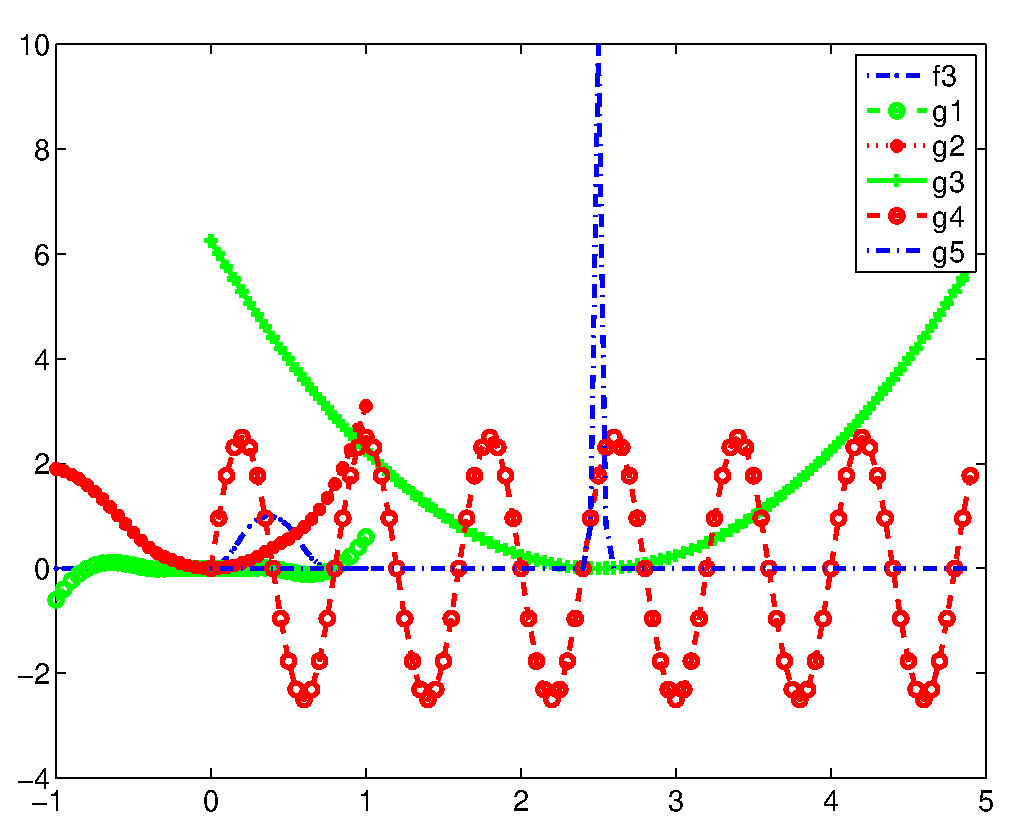
\includegraphics[width=59mm]{figure/traub_funappxNoPenalty_g_testfun.eps} & \hspace{-3ex}
\includegraphics[width=60mm]{figure/traub_funappxNoPenalty_g_test}
  \\ a)  & b) 
  \end{tabular}
\caption{a) Test functions for comparing \funappxg, \funappxglobalg, and
Chebfun. b)  Ratios of run time and number of nodes used by \funappxg{} to \funappxglobalg{} (LEFT)
to Chebfun (RIGHT). This figure is conditionally reproduced by
\texttt{traubpaper\_funappx\_g\_test.m}.}
  \label{fig:testfunctions}
\end{figure}

%
\begin{table}[bth]
\centering
\caption{Comparison of number of sample points, computational time, success and
failure rates of \funappxg, \funappxglobalg, and
Chebfun. We also report the number of warnings in parentheses issued by the
sofwtare. This table can be conditionally reproduced by
\texttt{traubpaper\_funappx\_g\_test.m}.}
\label{tab:localVsGlobalVsChebfun}
{\footnotesize
\setlength{\tabcolsep}{.13em} % set table width
\begin{tabular}{|c|rrr|rrr|rrrrrr|rr|}
\hline
    Test      &     \multicolumn{3}{c|}{Number of Points} & \multicolumn{3}{c|}{Time Used}  & \multicolumn{6}{|c|}{Success (\%)} &  \multicolumn{2}{c|}{Failure (\%)}
\\  functions &  Local  &  Global    &  Chebfun & Local       &  Global  & Chebfun              & \multicolumn{2}{c}{Local}   &  \multicolumn{2}{c}{Global}  & \multicolumn{2}{c}{Chebfun}  & \multicolumn{2}{|c|}{Chebfun}  
\\ \hline
      $g_1$ &   4152  &   30357  & 5069   &   0.052   &  0.030  &  3.989  &    100  & (100) &  100  &  (0) &     61 &   (24)  &    39  &  (39) 
\\    $g_2$ &   4223  &   51050  & 4720   &   0.057   &  0.038  &  3.563  &    100  & ( 72) &  100  &  (0) &    100 &   (51)  &     0  &  ( 0) 
\\    $g_3$ &    867  &   14640  &    4   &   0.046   &  0.014  &  0.094  &    100  & ( 34) &  100  &  (0) &     96 &   ( 0)  &     4  &  ( 0) 
\\    $g_4$ &   5011  &   46049  &    3   &   0.026   &  0.029  &  0.011  &    100  & (100) &  100  &  (0) &    100 &   ( 0)  &     0  &  ( 0) 
\\    $g_5$ &  29671  &  110027  &   37   &   0.059   &  0.032  &  0.016  &    100  & (  0) &  100  &  (0) &    100 &   ( 0)  &     0  &  ( 0) 
\\    $g_6$ &  11580  &  509263  &  127   &   0.037   &  0.138  &  0.129  &    100  & (100) &  100  &  (0) &     82 &   ( 0)  &    18  &  ( 0) 
\\ \hline
\end{tabular}
}
\end{table}
%

From Table~\ref{tab:localVsGlobalVsChebfun}, we see that both \funappxg{} and
\funappxglobalg{} achieved total success. The former worked better than
\funappxglobalg{} for all test cases in terms of \emph{average} number of run
time and number of sampling points. It was also more \emph{cautionary} since it
issued more warnings than \funappxglobalg.
%
In contrast, Chebfun generally used substantially less number of node points
than \funappxg{} even though the run time was not shorter in about~30\% of the
test cases; see Figure~\ref{fig:testfunctions}b)(RIGHT). However it was
particularly challenged by the highly oscillatory functions $g_1$ and $g_2$ in
terms of run time and success rates. In some instances of the peaky functions
$g_3$ and $g_6$, it failed to approximate them satisfactorily for about~10\% of
the cases.
\end{exmp} 

\begin{comment}
\begin{exmp}
In this example, we consider the function $f_4(x) = sin(10 \pi x^4) + x$, which
is increasing oscillating over the interval $[0,2]$. We use \funappxg, \funming,
and \integralg to approximate the function, locate its global minimum, and
estimate its integral with $\abstol = 10^{-8}$. With $1,972,359$ points,
\funappxg can approximate $f_4$ uniformly accurate as shown in
Figure~\ref{f4fig}(a). The true global minimum is $(0.6212340312,
-0.3782149854)$ and the absolute approximation error of \funming using
$n=2,022,621$ points is $(1.4\times 10^{-7}, 4.7\times 10^{-11})$. The integral
$\int_{0}^{2} f_4 (x) dx = 2.145517314$ and the approximation error of
\integralg is $4.7\times10^{-10}$ using $4,965,641$ points.

\begin{figure}[bt]
\centering
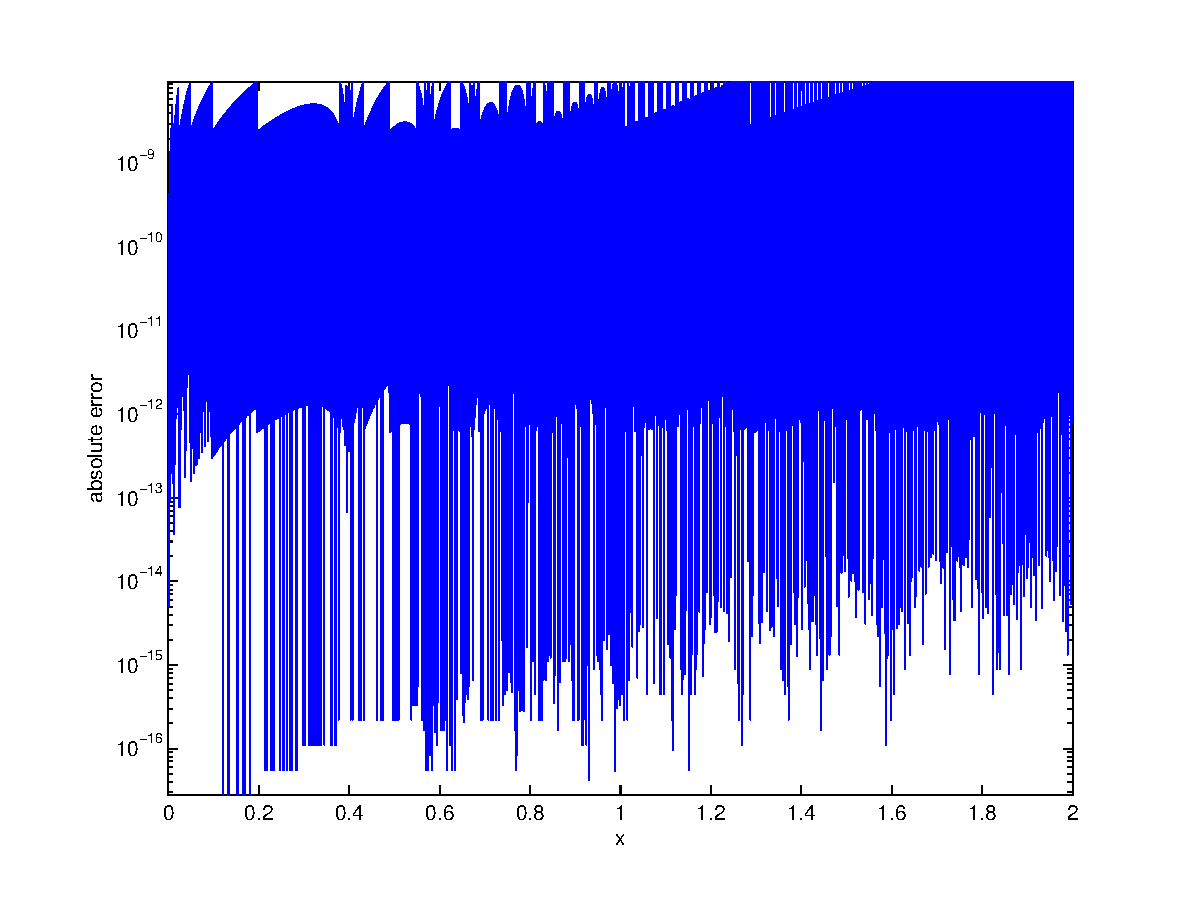
\includegraphics[width=6.2cm]{figure/f4_funappx_error.eps} \hspace{-5ex}
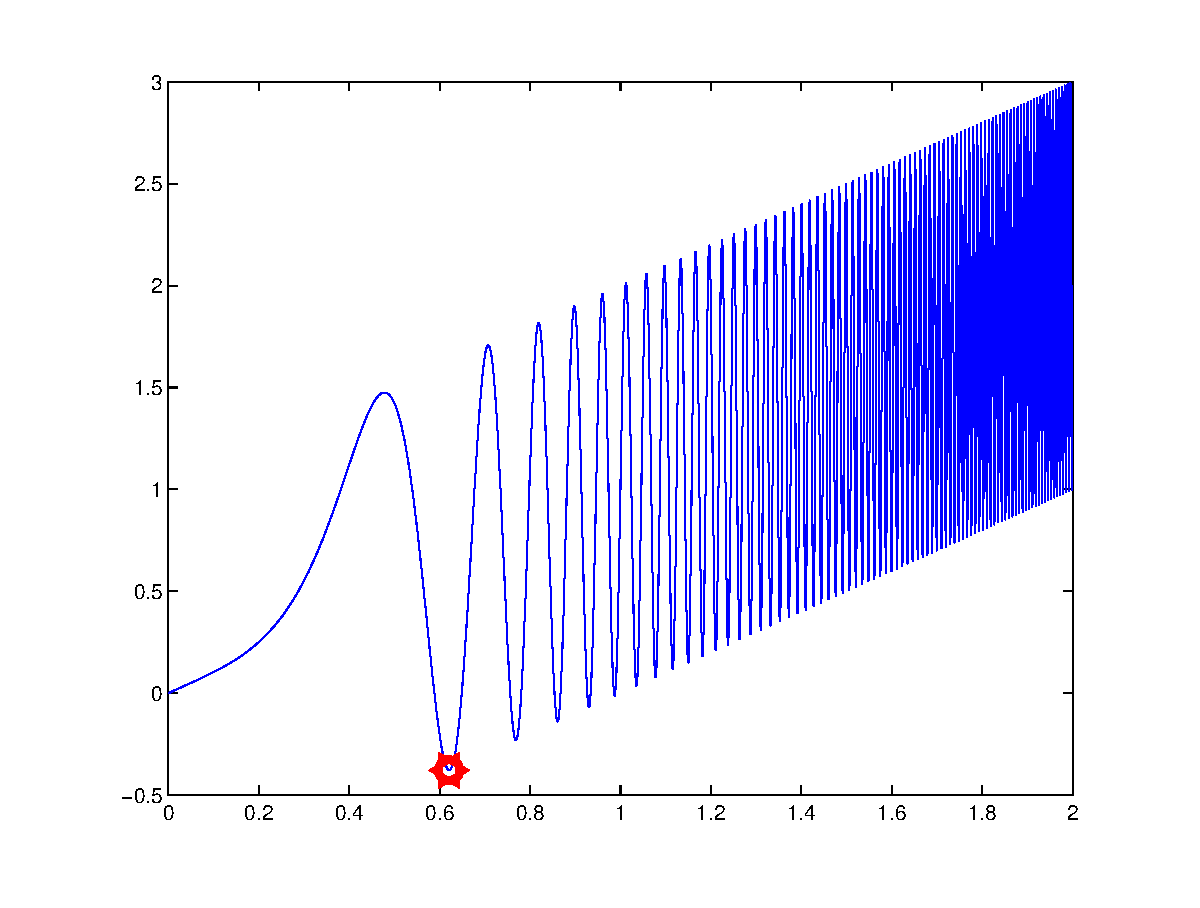
\includegraphics[width=6.2cm]{figure/f4_funmin_g.eps}
\caption{The example $f_4$ with errors of interpolants from \funappxg (left) and
minimum found by \funming (right).}
\label{f4fig}
\end{figure}
\end{exmp}
\end{comment}


     
\begin{comment}
Our algorithm is readily extensible to the following complex-valued function.
\begin{exmp}
This example is taken from MATLAB's documentation for \texttt{interp1}. Define
the complex valued function $v(x) = 5x + x^2 i$ for $x \in [1,10]$. It is clear
that the real part of $v$ is $5x$ and the imaginary part is $x^2$. We could
apply \funappxg to approximate the two parts separately. However, it is
unnecessary.
\end{exmp}
\end{comment}

 

